\setcounter{chapter}{10}  % sets the current chapter to 10 so that the next one becomes 11

\chapter{Introduction to Hypothesis Testing}
\label{ch:intro-hypothesis}

\section{Test of Hypothesis for One Mean}

\begin{definition}[Hypothesis Tests]
An inferential procedure to determine whether there is sufficient evidence to suggest a condition for a population parameter using statistics from a sample.
\end{definition}


\textcolor{blue}{Attach a probability to the conclusion of a hypothesis test.}

\subsubsection*{Steps}
\begin{enumerate}
    \item Decide on a level of significance ($\alpha$)
    \item State the null hypothesis ($H_0$) and the alternative hypothesis ($H_a$) \textcolor{blue}{($H_1$)}
    \item Calculate the appropriate test statistic.
    \item Use the test statistic and a reference distribution to calculate a p-value. \\
    \textcolor{blue}{(Also refer back to $H_a$)}
    \item Compare p-value to $\alpha$ to make a conclusion.
\end{enumerate}

\textcolor{blue}{Note:} \\
\textcolor{blue}{The definition of a p-value can be confusing. We will define it later.}

\subsection*{Step 1: Decide on a Level of Significance ($\alpha$)}
-Threshold for decision making.

-Depends on tolerance for consequences of errors, sample size, nature of the study, and variability.

-Common values: $0.10$, $0.01$, $0.05$ \textcolor{blue}{(very common default)}

\subsection*{Step 2: State the Null Hypothesis ($H_0$) and the Alternative Hypothesis ($H_a$)}

\textbf{$\Theta$:} parameter of interest

\textbf{$\Theta_0$:} numerical value of the parameter of interest hypothesized under the null hypothesis.

\[
\begin{array}{lll}
H_0: \Theta = \Theta_0 & (\Theta \leq \Theta_0) & H_a: \Theta > \Theta_0 \quad \textcolor{blue}{\text{one-sided (one-tailed)}} \\
H_0: \Theta = \Theta_0 & (\Theta \geq \Theta_0) & H_a: \Theta < \Theta_0 \quad \textcolor{blue}{\text{one-sided (one-tailed)}} \\
H_0: \Theta = \Theta_0 &                         & H_a: \Theta \neq \Theta_0 \quad \textcolor{purple}{\text{two-sided (two-tailed)}}
\end{array}
\]


\textbf{Null ($H_0$):} Represents the current belief (\textcolor{blue}{status quo}) or the safe belief.

\textbf{Alternative ($H_a$):} Represents the research hypothesis (or what you are asked to test)
\subsection*{Step 3: Calculate an appropriate test statistic}

Depends on the hypothesis test conducted and the information available.


\begin{definition}[Test Statistic Skeleton]
\[
\text{test statistic} = \frac{\text{(a statistic)} - \text{(hypothesized value of parameters under } H_0 \text{)}}{\text{standard error of statistic}}
\]
\end{definition}

The test statistic follows a reference distribution ($Z$, $t$, $F$, $\chi^2$).
\subsection*{Step 4: Calculate the p-value}

\noindent
Use the test statistic, reference distribution, and refer back to $H_a$.

% --- BLUE: Right-tailed tests ---
\begin{figure}[H]
  \centering
  \begin{minipage}[t]{0.48\textwidth}
    \centering
    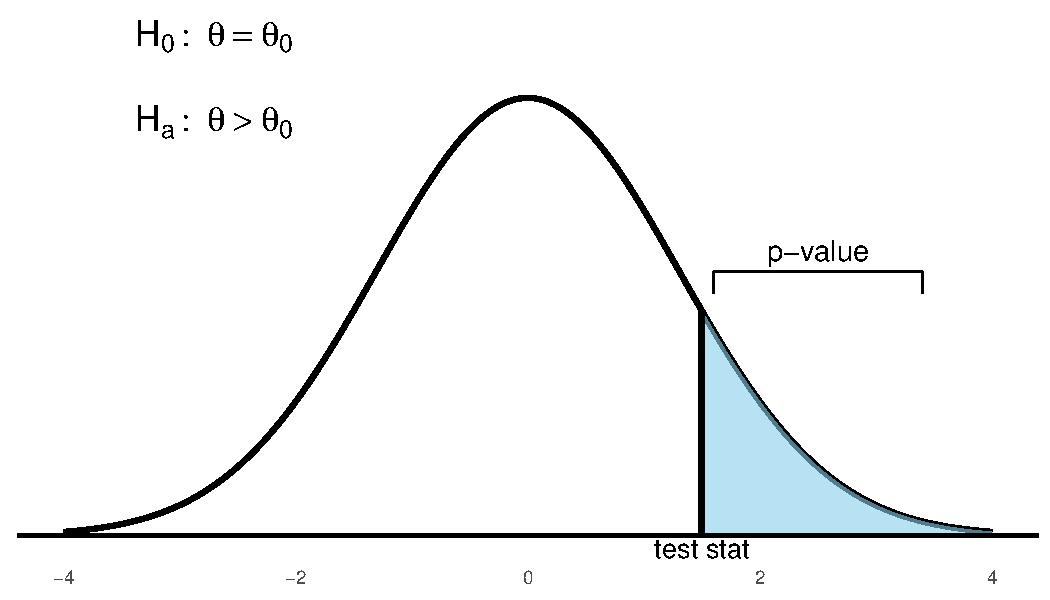
\includegraphics[width=\linewidth]{section11/images/hypothesis_right_tail.pdf}
  \end{minipage}
  \hfill
  \begin{minipage}[t]{0.48\textwidth}
    \centering
    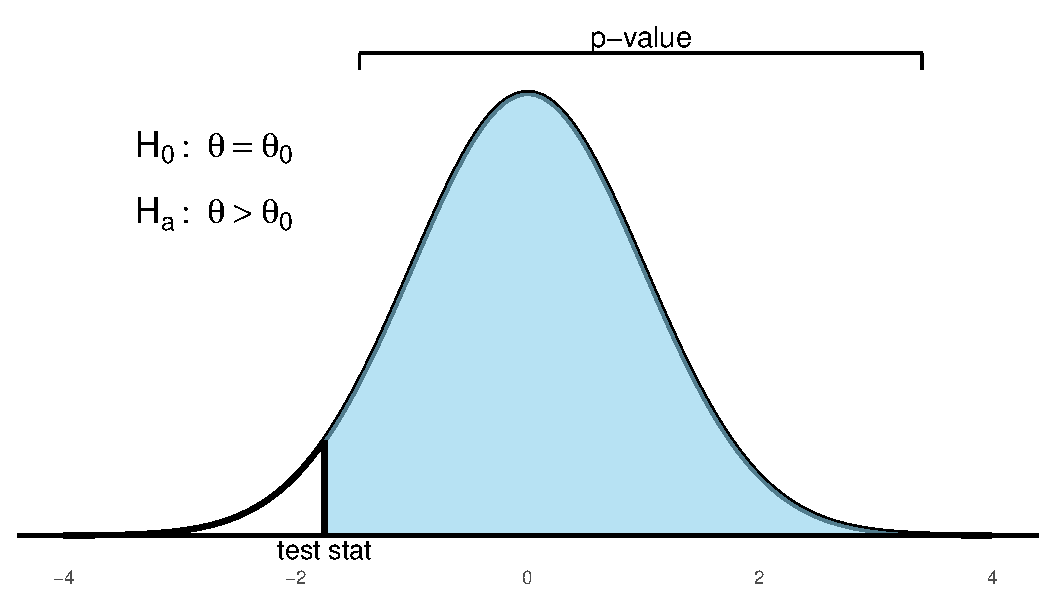
\includegraphics[width=\linewidth]{section11/images/hypothesis_right_tail_wide.pdf}
  \end{minipage}
  \caption*{Right-tailed test: \textit{p}-value is the area to the right of the test statistic.}
\end{figure}


% --- PINK: Left-tailed tests ---
\begin{figure}[H]
  \centering
  \begin{minipage}{0.48\textwidth}
    \centering
    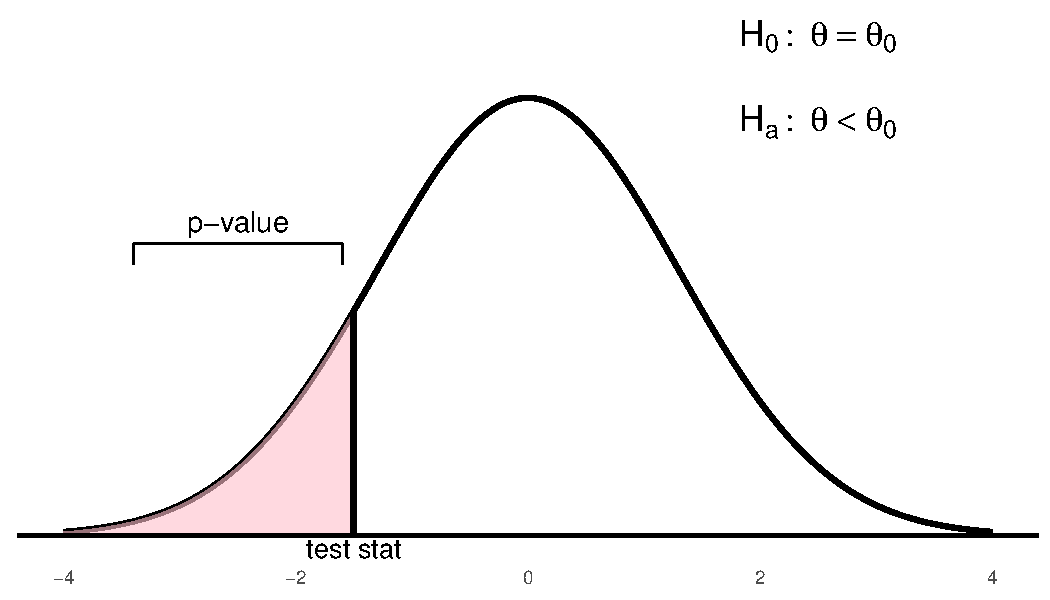
\includegraphics[width=\textwidth]{section11/images/hypothesis_left_tail.pdf}
  \end{minipage}
  \hfill
  \begin{minipage}{0.48\textwidth}
    \centering
    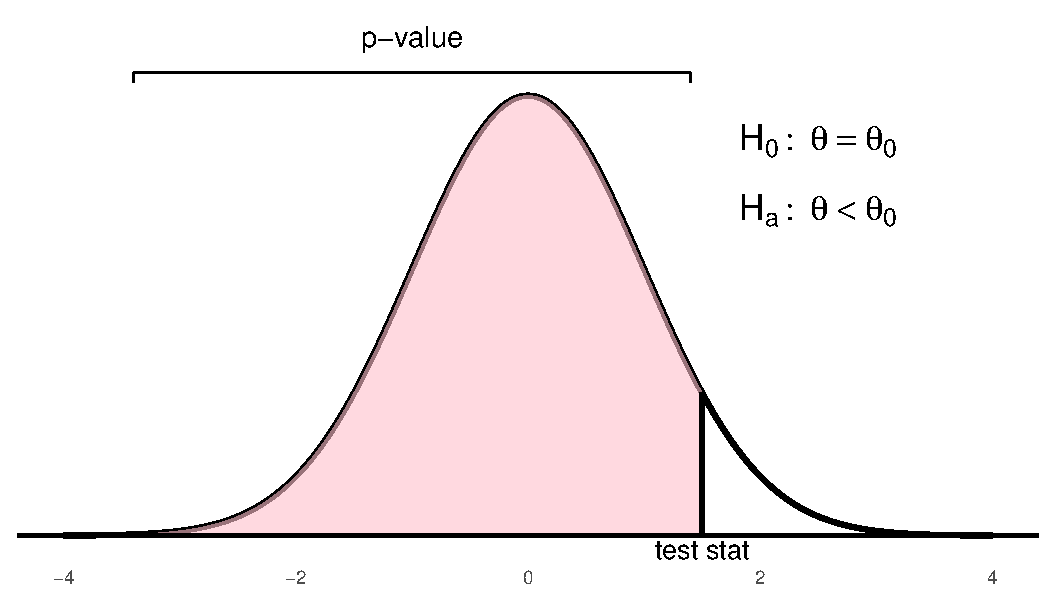
\includegraphics[width=\textwidth]{section11/images/hypothesis_left_tail_wide.pdf}
  \end{minipage}
\caption*{Left-tailed test: \textit{p}-value is the area to the left of the test statistic.}
\end{figure}

% --- GREEN: Two-tailed test ---
\begin{figure}[H]
  \centering
  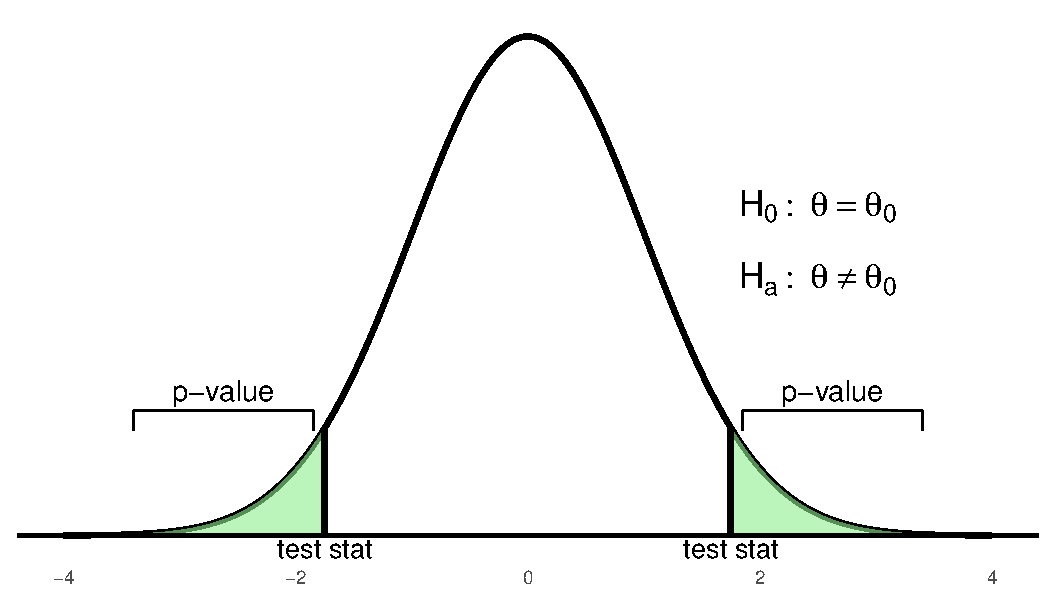
\includegraphics[width=0.52\textwidth]{section11/images/hypothesis_two_tail.pdf}
  \caption*{Two-tailed test: p-value is the total area in both tails beyond $\pm$ test statistic.}
\end{figure}
\subsection*{Step 5: Compare \textit{p}-value to level of significance $\alpha$ and make a conclusion}

\begin{itemize}
  \item If \textit{p}-value $< \alpha$: \\
  \quad Sufficient evidence against $H_0$. The hypothesis test rejects $H_0$ in favor of $H_a$.

  \item If \textit{p}-value $> \alpha$: \\
  \quad Insufficient evidence against $H_0$. Do not reject $H_0$ (fail to reject $H_0$).
\end{itemize}

\textbf{Note:} It is not good practice to give conclusions in the context of stating we \textit{accept $H_0$} or \textit{accept $H_a$}.
\begin{example}[Sweetening Colas]
Diet colas use artificial sweeteners to avoid sugar. These sweeteners gradually lose their sweetness over time. Manufacturers therefore test new colas for loss of sweetness before marketing them. Trained tasters sip the cola along with drinks of standard sweetness and score the cola on a “sweetness score” of 1 to 10. The cola is then stored for a month at high temperature to imitate the effect of four months’ storage at room temperature. Each taster scores the cola again after storage. This is a matched pairs experiment. Our data are the differences (score before storage minus score after storage) in the tasters’ scores. The bigger these differences, the bigger the loss of sweetness.

Suppose we know that for any cola, the sweetness loss scores vary from taster to taster according to a Normal distribution with standard deviation $\sigma = 1$. The mean $\mu$ for all tasters measures loss of sweetness.

The following are the sweetness losses for a new cola as measured by 10 trained tasters:

\medskip
\centerline{2.0,\ 0.4,\ 0.7,\ 2.0,\ -0.4,\ 2.2,\ -1.3,\ 1.2,\ 1.1,\ 2.3}
\medskip

Are these data good evidence that the cola lost sweetness in storage?\\
\noindent\textbf{Solution}\\

$\mu$ = mean sweetness loss for the population of \textbf{all} tasters.\\
\textbf{Step 1:} State hypotheses. $H_0: \mu = 0$ vs $H_a: \mu > 0$ \\
\textbf{Step 2:} Test statistic: $z_\star = \dfrac{\bar{x} - \mu_0}{\sigma / \sqrt{n}} = \dfrac{1.02 - 0}{1 / \sqrt{10}} = 3.23$ \\
\textbf{Step 3:} P-value. $P(Z > z_\star) = P(Z > 3.23) = 0.0006$ \\
\textbf{Step 4:} Conclusion. We would rarely observe a mean as large as 1.02 if $H_0$ were true. The small p-value provides strong evidence against $H_0$, supporting $H_a: \mu > 0$. That is, the mean sweetness loss is likely positive.

\vspace{1em}
\noindent\textbf{R code (Simulation)}

\begin{tcolorbox}[colback=gray!10, colframe=black!45, arc=2mm]
\begin{verbatim}
# n = sample size;
n<-10;
mu.zero<-0;
sigma<-1;
sigma.xbar<-sigma/sqrt(n);

# x bar = sample mean with 10 obs;
x.bar<-rnorm(1,mean=mu.zero,sd=sigma.xbar);
x.bar;

## [1] 0.3265859

# z.star = test statistic;
z.star<-(x.bar-mu.zero)/sigma.xbar;
z.star;

## [1] 1.032755
\end{verbatim}
\end{tcolorbox}
\vspace{1em}
\noindent\textbf{R code (10,000 Simulations)}

\begin{tcolorbox}[colback=gray!10, colframe=black!45, arc=2mm]
\begin{verbatim}
n <- 10;
mu.zero <- 0;
sigma <- 1;
sigma.xbar <- sigma / sqrt(n);
# x bar = sample mean with 10 obs;
# m = number of simulations;
m <- 10000;
x.bar <- rnorm(m, mean = mu.zero, sd = sigma.xbar);

# z.star = test statistic;
z.star <- (x.bar - mu.zero) / sigma.xbar;
hist(z.star, xlab = "differences", col = "blue");
\end{verbatim}
\end{tcolorbox}
\vspace{1em}
\noindent\textbf{Histogram from simulation (see Section 7 for R code format)}

\begin{figure}[H]
  \centering
  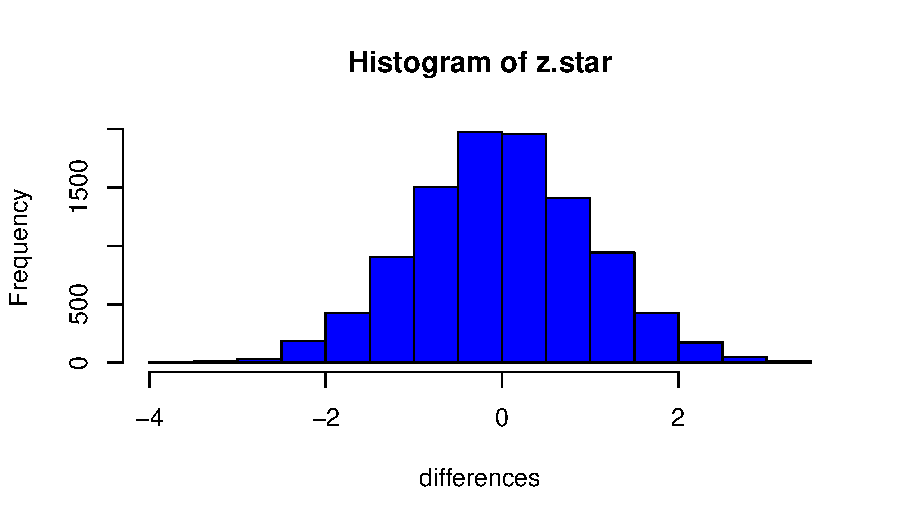
\includegraphics[width=0.6\textwidth]{Section11/images/sweetening_10000_hist.pdf}
  \caption*{Histogram of $z_\star$ values from 10,000 simulations under $H_0$.}
\end{figure}
\vspace{1em}
\noindent\textbf{R code (Empirical p-value)}

\begin{tcolorbox}[colback=gray!10, colframe=black!45, arc=2mm]
\begin{verbatim}
## P-value

p_value <- length(z.star[z.star > 3.23]) / m;

p_value

## [1] 8e-04
\end{verbatim}
\end{tcolorbox}


\end{example}
\begin{tcolorbox}[colback=yellow!5, colframe=yellow!50!black, title={One-Sample Hypothesis Test for Population Mean ($\mu$)}, sharp corners, boxrule=0.4pt, width=\textwidth, breakable]
\textbf{When $\sigma$ is known:}

\begin{tabular}{@{}ll@{\hspace{1.2cm}}ll@{}}
$\bullet\ H_0\!: \mu = \mu_0$ & (or $\mu \leq \mu_0$) & $H_a\!: \mu > \mu_0$ \\
$\bullet\ H_0\!: \mu = \mu_0$ & (or $\mu \geq \mu_0$) & $H_a\!: \mu < \mu_0$ \\
$\bullet\ H_0\!: \mu = \mu_0$ & & $H_a\!: \mu \neq \mu_0$ \\
\end{tabular}

\vspace{0.75em}
\begin{tabular}{@{}l l@{}}
\textbf{Test statistic:} & $z^* = \dfrac{\bar{X} - \mu_0}{\sigma/\sqrt{n}}$
\end{tabular}


\vspace{0.75em}
\textbf{Reference distribution:} Standard normal ($Z$)
\end{tcolorbox}
\begin{example}[UTM Deer]
Deer are a common sight on the UTM campus. Suppose an ecologist is interested in the average mass of adult white-tailed does (female deer) around the Mississauga campus to determine whether they are healthy for the upcoming winter. The ecologist captures a sample of 36 adult females around the UTM and measures the average mass of this sample to be 42.53 kg.

From previous studies conducted in the area, the average mass of healthy does was reported to be 45 kg. Conduct a hypothesis test at the 5\% significance level to determine whether the mass of does around UTM has decreased. Assume the standard deviation is known to be 5.25 kg.


\vspace{1em}

\textbf{1. Level of significance.} \(\alpha = 0.05\)

\textbf{2. State the null and alternative hypotheses.}
\[
H_0: \mu = 45 \qquad H_a: \mu < 45
\]

\textbf{3. Calculate appropriate test statistic.}

\vspace{0.5em}

Given:
\[
n = 36, \quad \bar{x} = 42.53, \quad \sigma = 5.25
\]

Since \(\sigma\) is known, the test statistic is:
\[
z^* = \frac{\bar{x} - \mu_0}{\sigma / \sqrt{n}} = \frac{42.53 - 45}{5.25/\sqrt{36}} = -2.82
\]

Reference distribution: standard normal

\textbf{4. Calculate p-value}

\[
\text{p-value} = P(Z < -2.82) \approx 0.0024
\]

\captionsetup{skip=0pt} % no vertical gap between figure and caption
\begin{figure}[H]
\centering
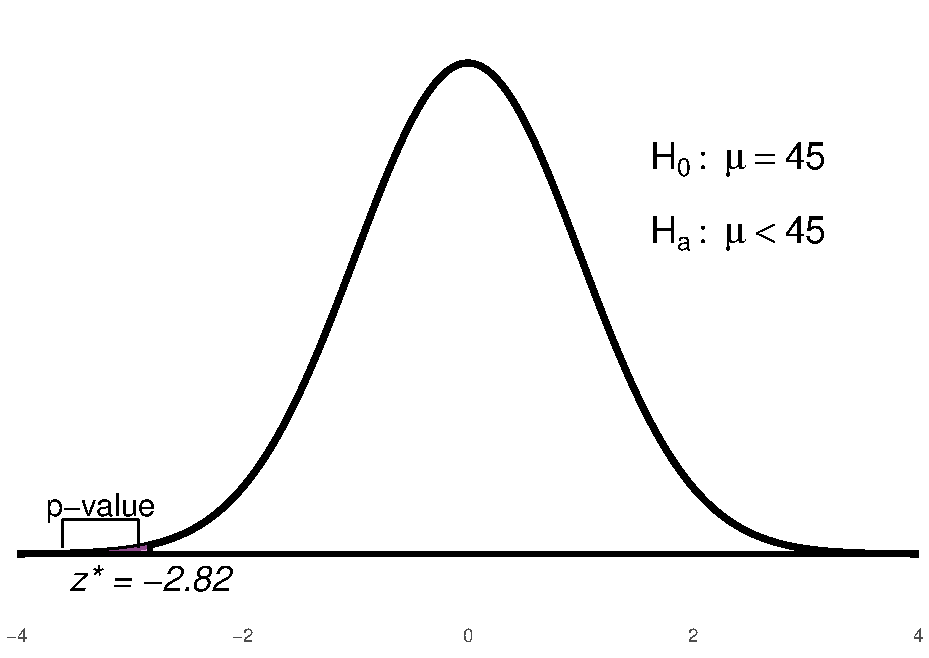
\includegraphics[width=0.6\textwidth]{section11/images/deer_pvalue.pdf}
\caption{Left-tailed p-value for the test statistic \( z^* = -2.82 \)}
\end{figure}

\textbf{5. Compare p-value with level of significance \(\alpha\) and make a conclusion:}

\[
0.0024 < 0.05 \Rightarrow \text{p-value} < \alpha
\]

There is sufficient evidence at the 5\% level of significance to reject the null that does this winter weigh the same as in the past and to conclude the alternative that does this winter weigh less than 45 kg.

\vspace{1em} % optional, if there's space needed above the label
\noindent\textbf{R code:}
\vspace{0.8em}
\begin{tcolorbox}[
  colback=gray!10, 
  colframe=black!45, 
  arc=2mm, 
  breakable, 
  after skip=0pt,  % no space after box
  before skip=0.3pt, % 🟢 key to tighten gap before box
  boxsep=1pt, left=4pt, right=4pt, top=2pt, bottom=2pt % 🟢 shrink padding
]
\begin{verbatim}
# Find test stat
z_test_stat = (42.53 - 45) / (5.25 / sqrt(36))
z_test_stat
[1] -2.822857

# Find the p-value
# Since the alternative is Ha : mu < 45
p-value = pnorm(z_test_stat)
[1] 0.00237989
\end{verbatim}
\end{tcolorbox}
\noindent\textit{Note:} The \texttt{pnorm()} function in R, by default, returns the cumulative probability (area) to the left of the given value. \\
\par\vspace{0.8em}  % <-- This forces the vertical break and then adds space
\noindent\textbf{R code: Using BSDA package}
\vspace{0.3em}

\begin{tcolorbox}[colback=gray!10, colframe=black!45, arc=2mm,
  breakable, boxsep=1pt, left=4pt, right=4pt, top=2pt, bottom=2pt,
  before skip=0pt, after skip=1em]
\small
\begin{verbatim}
# Using the BSDA library. install BSDA if it is not already installed.
# install.packages("BSDA")
> library(BSDA)
> # Conduct the z-test with the zsum.test function
> zsum.test(mean.x = 42.53, sigma.x = 5.24, n.x = 36, mu = 45, alternative = "less")

        One-sample z-Test

data:  Summarized x
z = -2.8282, p-value = 0.00234
alternative hypothesis: true mean is less than 45
95 percent confidence interval:
 NA 43.96651
sample estimates:
mean of x 
    42.53 
\end{verbatim}
\end{tcolorbox}

\vspace{1em}
\noindent\textbf{Interpretation:}

There is sufficient evidence at the 5\% level of significance to reject the null hypothesis. We conclude that the average mass of does this winter is significantly less than 45 kg.
\end{example}

\begin{example}[Executives’ Blood Pressures]

The National Center for Health Statistics reports that the systolic blood pressure for males 35 to 44 years of age has mean 128 and standard deviation 15. 

The medical director of a large company looks at the medical records of 72 executives in this age group and finds that the mean systolic blood pressure in this sample is $\bar{x} = 126.07$. Is this evidence that the company’s executives have a different mean blood pressure from the general population?

Suppose we know that executives’ blood pressures follow a Normal distribution with standard deviation $\sigma = 15$.

\textbf{Solution:} Let $\mu$ be the mean systolic blood pressure of the executive population.

\begin{enumerate}
    \item \textbf{State hypotheses:} \\
    $H_0: \mu = 128$ \hspace{1cm} vs \hspace{1cm} $H_a: \mu \ne 128$
    
    \item \textbf{Test statistic:} \\
    \[
    z_\ast = \frac{\bar{x} - \mu_0}{\sigma / \sqrt{n}} = \frac{126.07 - 128}{15 / \sqrt{72}} = -1.09
    \]

    \item \textbf{P-value:} \\
    \[
    2P(Z > |z_\ast|) = 2P(Z > 1.09) = 2(1 - 0.8621) = 0.2758
    \]

    \item \textbf{Conclusion:} \\
    More than 27\% of the time, a simple random sample of size 72 from the general male population would have a mean blood pressure at least as far from 128 as that of the executive sample. The observed $\bar{x} = 126.07$ is therefore not good evidence that executives differ from other men.
\end{enumerate}

\end{example}
\begin{tcolorbox}[title=\textbf{Tests for a Population Mean},
  colback=yellow!10,
  colframe=black!45,
  coltitle=black,
  fonttitle=\bfseries,
  breakable]

There are four steps in carrying out a significance test:
\begin{enumerate}
  \item State the hypotheses.
  \item Calculate the test statistic.
  \item Find the P-value.
  \item State your conclusion in the context of your specific setting.
\end{enumerate}

Once you have stated your hypotheses and identified the proper test, you or your computer can do Steps 2 and 3 by following a recipe. 

\end{tcolorbox}
\begin{tcolorbox}[title=\textbf{Z Test for a Population Mean $\mu$},
  colback=yellow!10,
  colframe=black!45,
  coltitle=black,
  fonttitle=\bfseries,
  breakable]

Here is the recipe for the test we have used in our examples.\\
Draw a simple random sample of size $n$ from a Normal population that has unknown mean $\mu$ and known standard deviation $\sigma$.

To test the null hypothesis that $\mu$ has a specified value, $H_0 : \mu = \mu_0$, calculate the \textbf{one-sample $z$ statistic}:
\[
z_\ast = \frac{\bar{x} - \mu_0}{\sigma / \sqrt{n}}
\]

In terms of a variable $Z$ having the standard Normal distribution, the P-value for a test of $H_0$ against:
\begin{itemize}
  \item $H_a: \mu > \mu_0$ is $P(Z > z_\ast)$
  \item $H_a: \mu < \mu_0$ is $P(Z < z_\ast)$
  \item $H_a: \mu \ne \mu_0$ is $2P(Z > |z_\ast|)$
\end{itemize}

\end{tcolorbox}
\begin{example}

Consider the following hypothesis test:

\begin{align*}
H_0 &: \mu = 20 \\
H_a &: \mu < 20
\end{align*}


A sample of 50 provided a sample mean of 19.4. The population standard deviation is 2.

\begin{enumerate}
    \item[(a)] Compute the value of the test statistic.
    \item[(b)] What is the p-value?
    \item[(c)] Using $\alpha = 0.05$, what is your conclusion?
\end{enumerate}

\textbf{Solution:}

\begin{enumerate}
    \item[(a)] \textbf{Test statistic:}
    \[
    z_\ast = \frac{\bar{x} - \mu_0}{\sigma / \sqrt{n}} = \frac{19.4 - 20}{2 / \sqrt{50}} = -2.1213
    \]
    
    \item[(b)] \textbf{P-value:}
    \[
    P(Z < z_\ast) = P(Z < -2.1213) = 0.0169
    \]

    \item[(c)] \textbf{Conclusion:} \\
    Since the P-value $= 0.0169 < \alpha = 0.05$, we reject $H_0 : \mu = 20$. We conclude that $\mu < 20$.
\end{enumerate}

\end{example}
\begin{example}

Consider the following hypothesis test:

\begin{align*}
H_0 &: \mu = 25 \\
H_a &: \mu > 25
\end{align*}


A sample of 40 provided a sample mean of 26.4. The population standard deviation is 6.

\begin{enumerate}
    \item[(a)] Compute the value of the test statistic.
    \item[(b)] What is the p-value?
    \item[(c)] Using $\alpha = 0.01$, what is your conclusion?
\end{enumerate}

\textbf{Solution:}

\begin{enumerate}
    \item[(a)] \textbf{Test statistic:}
    \[
    z_\ast = \frac{\bar{x} - \mu_0}{\sigma / \sqrt{n}} = \frac{26.4 - 25}{6 / \sqrt{40}} = 1.4757
    \]

    \item[(b)] \textbf{P-value:}
    \[
    P(Z > z_\ast) = P(Z > 1.4757) = 0.0700
    \]

    \item[(c)] \textbf{Conclusion:} \\
    Since P-value $= 0.0700 > \alpha = 0.01$, we \textbf{cannot reject} $H_0 : \mu = 25$. \\
    We conclude that we don’t have enough evidence to claim that $\mu > 25$.
\end{enumerate}

\end{example}
\begin{example}

Consider the following hypothesis test:

\begin{align*}
H_0 &: \mu = 15 \\ 
H_a &: \mu \ne 15
\end{align*}

A sample of 50 provided a sample mean of 14.15. The population standard deviation is 3.

\begin{enumerate}
    \item[(a)] Compute the value of the test statistic.
    \item[(b)] What is the p-value?
    \item[(c)] Using $\alpha = 0.05$, what is your conclusion?
\end{enumerate}

\textbf{Solution:}

\begin{enumerate}
    \item[(a)] \textbf{Test statistic:}
    \[
    z_\ast = \frac{\bar{x} - \mu_0}{\sigma / \sqrt{n}} = \frac{14.15 - 15}{3 / \sqrt{50}} = -2.0034
    \]

    \item[(b)] \textbf{P-value:}
    \[
    2P(Z > |z_\ast|) = 2P(Z > |{-2.0034}|) = 2P(Z > 2.0034) = 0.0451
    \]

    \item[(c)] \textbf{Conclusion:} \\
    Since P-value $= 0.0451 < \alpha = 0.05$, we reject $H_0 : \mu = 15$. \\
    We conclude that $\mu \ne 15$.
\end{enumerate}

\textbf{Confidence Interval Interpretation:}

The 95\% confidence interval for $\mu$ is:
\[
\bar{x} \pm z_\ast \left( \frac{\sigma}{\sqrt{n}} \right)
\]
\[
14.15 \pm 1.96 \left( \frac{3}{\sqrt{50}} \right)
= (13.3184,\ 14.9815)
\]

Since the hypothesized value $\mu_0 = 15$ falls \textbf{outside} this interval, we again reject $H_0 : \mu = 15$.

\end{example}
\begin{nt}[Confidence Intervals and Two-Sided Tests]
\textit{
A level $\alpha$ two-sided significance test rejects a hypothesis $H_0 : \mu = \mu_0$ exactly when the value $\mu_0$ falls outside a level $1 - \alpha$ confidence interval for $\mu$.
}

\end{nt}
\begin{tcolorbox}[colback=yellow!5, colframe=yellow!50!black, 
  title={One-Sample Hypothesis Test for Population Mean ($\mu$) \textbf{(When $\sigma$ is not known)}},
  sharp corners, boxrule=0.4pt, width=\textwidth, breakable]

\begin{tabular}{@{}ll@{\hspace{1.2cm}}ll@{}}
$\bullet$ H$_0\!$: $\mu = \mu_0$ & (or $\mu \geq \mu_0$) & $H_a\!$: $\mu < \mu_0$ \\
$\bullet$ H$_0\!$: $\mu = \mu_0$ & (or $\mu \leq \mu_0$) & $H_a\!$: $\mu > \mu_0$ \\
$\bullet$ H$_0\!$: $\mu = \mu_0$ & & $H_a\!$: $\mu \ne \mu_0$
\end{tabular}

\vspace{0.75em}
\begin{tabular}{@{}l @{}}
\textbf{Test statistic:} $t^\ast = \dfrac{\bar{X} - \mu_0}{s / \sqrt{n}}$
\end{tabular}

\vspace{0.75em}
\textbf{Reference distribution:} $t$ distribution with $n - 1$ degrees of freedom

\end{tcolorbox}
\begin{example}[Hypothesis Test: Laughter and Heart Rate, Unknown $\sigma$]

Researchers studied the physiological effects of laughter. They measured heart rates (in beats per minute) of \textbf{$n = 25$} subjects (ages 18–34) while they laughed. They obtained:
\[
\bar{x} = 73.5, \quad s = 6, \quad \alpha = 0.05
\]
It is well known that the resting heart rate is 71 bpm. Is there evidence that the mean heart rate during laughter exceeds 71 bpm?

\textbf{Step 1: State the hypotheses.}
\[
\begin{aligned}
H_0 &: \mu = 71 \\
H_a &: \mu > 71
\end{aligned}
\]

\textbf{Step 2: Check assumptions.}
\begin{itemize}
  \item The sample is an independent random sample of individuals aged 18–34.
  \item The population of heart rates during laughter is normally distributed.
\end{itemize}

\textbf{Step 3: Compute the test statistic.}

Since $\sigma$ is unknown, we use the $t$ statistic:
\[
t^\ast = \frac{\bar{x} - \mu_0}{s / \sqrt{n}} = \frac{73.5 - 71}{6 / \sqrt{25}} = 2.083
\]

Reference distribution: $t$ distribution with $n - 1 = 25 - 1 = 24$ degrees of freedom.

\textbf{Step 4: Determine the p-value.}

Using the $t$ distribution with 24 df:
\[
0.01 < \text{p-value} < 0.025
\]

\textbf{Step 5: Make a conclusion.}

Since $\text{p-value} < \alpha = 0.05$, we reject $H_0$.

\textit{There is sufficient evidence at the 5\% level of significance to reject the null that the mean is 71 bpm in favor of the alternative that the mean is greater than 71 bpm for people who are laughing.}


\end{example}
\begin{example}

A researcher is asked to test the hypothesis that the average price of a 2-star (CAA rating) motel room has decreased since last year. Last year, a study showed that the prices were Normally distributed with a mean of \$89.50.

A random sample of twelve 2-star motels produced the following room prices:

\[
\text{\$85.00, 92.50, 87.50, 89.90, 90.00, 82.50, 87.50, 90.00, 85.00, 89.00, 91.50, 87.50}
\]

At the 5\% level of significance, can we conclude that the mean price has decreased?

\textbf{Solution:}

Let $\mu$ be the true average price of a 2-star motel room.

\begin{enumerate}
  \item \textbf{State hypotheses.}
  \[
  H_0 : \mu = 89.5 \quad \text{vs} \quad H_a : \mu < 89.5
  \]

  \item \textbf{Compute test statistic.}
  \[
  t^\ast = \frac{\bar{x} - \mu_0}{s / \sqrt{n}} = \frac{88.1583 - 89.5}{2.9203 / \sqrt{12}} = -1.5915
  \]

  \item \textbf{Find the P-value.} \\
  With $df = 11$, the P-value (from the $t$-distribution table) is between 0.05 and 0.10.

  \item \textbf{Conclusion.} \\
  Since P-value $> 0.05$, we \textbf{fail to reject} $H_0$. \\
  There is not sufficient evidence to conclude that the average price of 2-star motels has decreased this year.
\end{enumerate}
\vspace{1em}
\noindent\textbf{R code (One Sample t-test)}
\begin{tcolorbox}[colback=gray!10, colframe=black!45, arc=2mm]
\begin{verbatim}
# Step 1. Entering data;
prices=c(85.00, 92.50, 87.50, 89.90, 90.00, 82.50,
         87.50, 90.00, 85.00, 89.00, 91.50, 87.50);

# Step 2. Hypothesis test;
t.test(prices, alternative="less", mu=89.5);
\end{verbatim}
\end{tcolorbox}
\vspace{1em}
\noindent\textbf{R output}
\begin{tcolorbox}[colback=gray!10, colframe=black!45, arc=2mm]
\begin{verbatim}
## 
##  One Sample t-test
## 
## data:  prices
## t = -1.5915, df = 11, p-value = 0.0699
## alternative hypothesis: true mean is less than 89.5
## 95 percent confidence interval:
##  -Inf 89.67229
## sample estimates:
## mean of x 
##  88.15833 
\end{verbatim}
\end{tcolorbox}


\end{example}

\begin{tcolorbox}[title=\textbf{The one-sample \textit{t} test},
  colback=yellow!10,
  colframe=black!45,
  coltitle=black,
  fonttitle=\bfseries,
  breakable]

Draw an SRS of size $n$ from a large population having unknown mean $\mu$.

To \textit{test the hypothesis} $H_0 : \mu = \mu_0$, compute the \textit{one-sample $t$ statistic}
\[
t^\ast = \frac{\bar{x} - \mu_0}{s / \sqrt{n}}
\]

In terms of a variable $T$ having the $t_{n - 1}$ distribution, the P-value for a test of $H_0$ against

\begin{align*}
H_a : \mu > \mu_0 &\quad \text{is} \quad P(T \ge t^\ast) \\
H_a : \mu < \mu_0 &\quad \text{is} \quad P(T \le t^\ast) \\
H_a : \mu \ne \mu_0 &\quad \text{is} \quad 2P(T \ge |t^\ast|)
\end{align*}

These P-values are exact if the population distribution is Normal and are approximately correct for large $n$ in other cases.

\end{tcolorbox}








